\documentclass{article}

\def\ParSkip{} 
% Packages
\usepackage{amssymb,amsmath,amsthm,bbm}
\usepackage{verbatim,float,url,dsfont}
\usepackage{graphicx,subfigure,psfrag}
\usepackage{algorithm,algorithmic}
\usepackage{mathtools,enumitem}
\usepackage{multirow}
\usepackage{ragged2e}
\usepackage{xr-hyper}
\usepackage{array}

\usepackage[colorlinks=true,citecolor=blue,urlcolor=blue,linkcolor=blue]{hyperref}
\usepackage[margin=1in]{geometry}
\usepackage[round]{natbib}

\usepackage[utf8]{inputenc} % allow utf-8 input
\usepackage[T1]{fontenc}    % use 8-bit T1 fonts
\usepackage{booktabs}       % professional-quality tables
\usepackage{nicefrac}         % compact symbols for 1/2, etc.
\usepackage{microtype}      % microtypography

\ifdefined\TimesFont 
\usepackage{times} % use times font
\fi

\ifdefined\ParSkip 
\usepackage{parskip} % use par skip
\fi

% Theorems and such
\newtheorem{theorem}{Theorem}
\newtheorem{lemma}{Lemma}
\newtheorem{corollary}{Corollary}
\newtheorem{proposition}{Proposition}
\theoremstyle{definition}
\newtheorem{remark}{Remark}
\newtheorem{definition}{Definition}

% Assumption
\newtheorem*{assumption*}{\assumptionnumber}
\providecommand{\assumptionnumber}{}
\makeatletter
\newenvironment{assumption}[2]{
  \renewcommand{\assumptionnumber}{Assumption #1#2}
  \begin{assumption*}
  \protected@edef\@currentlabel{#1#2}}
{\end{assumption*}}
\makeatother

% Widebar
\makeatletter
\newcommand*\rel@kern[1]{\kern#1\dimexpr\macc@kerna}
\newcommand*\widebar[1]{%
  \begingroup
  \def\mathaccent##1##2{%
    \rel@kern{0.8}%
    \overline{\rel@kern{-0.8}\macc@nucleus\rel@kern{0.2}}%
    \rel@kern{-0.2}%
  }%
  \macc@depth\@ne
  \let\math@bgroup\@empty \let\math@egroup\macc@set@skewchar
  \mathsurround\z@ \frozen@everymath{\mathgroup\macc@group\relax}%
  \macc@set@skewchar\relax
  \let\mathaccentV\macc@nested@a
  \macc@nested@a\relax111{#1}%
  \endgroup
}
\makeatother

% Min and max 
\DeclareMathOperator*{\argmin}{argmin}
\DeclareMathOperator*{\argmax}{argmax}
\DeclareMathOperator*{\minimize}{minimize}
\DeclareMathOperator*{\maximize}{maximize}
\DeclareMathOperator*{\find}{find}
\DeclareMathOperator{\st}{subject\,\,to}

% Other operators
\DeclareMathOperator{\Cov}{Cov}
\DeclareMathOperator{\Var}{Var}
\DeclareMathOperator{\dm}{dim}
\DeclareMathOperator{\col}{col}
\DeclareMathOperator{\row}{row}
\DeclareMathOperator{\nul}{null}
\DeclareMathOperator{\rank}{rank}
\DeclareMathOperator{\nuli}{nullity}
\DeclareMathOperator{\spa}{span}
\DeclareMathOperator{\sign}{sign}
\DeclareMathOperator{\supp}{supp}
\DeclareMathOperator{\diag}{diag}
\DeclareMathOperator{\aff}{aff}
\DeclareMathOperator{\conv}{conv}
\DeclareMathOperator{\dom}{dom}
\DeclareMathOperator{\tr}{tr}
\DeclareMathOperator{\df}{df}

% Other shortcuts 
\def\R{\mathbb{R}}
\def\C{\mathbb{C}}
\def\E{\mathbb{E}}
\def\P{\mathbb{P}}
\def\T{\mathsf{T}}
\def\half{\frac{1}{2}}
\def\df{\mathrm{df}}
\def\hy{\hat{y}}
\def\hf{\hat{f}}
\def\hmu{\hat{\mu}}
\def\halpha{\hat{\alpha}}
\def\hbeta{\hat{\beta}}
\def\htheta{\hat{\theta}}
\def\indep{\perp\!\!\!\perp}
\def\th{^{\textnormal{th}}}

\def\cA{\mathcal{A}}
\def\cB{\mathcal{B}}
\def\cD{\mathcal{D}}
\def\cE{\mathcal{E}}
\def\cF{\mathcal{F}}
\def\cG{\mathcal{G}}
\def\cK{\mathcal{K}}
\def\cH{\mathcal{H}}
\def\cI{\mathcal{I}}
\def\cL{\mathcal{L}}
\def\cM{\mathcal{M}}
\def\cN{\mathcal{N}}
\def\cP{\mathcal{P}}
\def\cS{\mathcal{S}}
\def\cT{\mathcal{T}}
\def\cW{\mathcal{W}}
\def\cX{\mathcal{X}}
\def\cY{\mathcal{Y}}
\def\cZ{\mathcal{Z}}


\title{Lecture 6: Autoregressive Integrated Moving Average Models \\ \smallskip  
\large Introduction to Time Series, Fall 2023 \\ \smallskip
Ryan Tibshirani}
\date{}

\begin{document}
\maketitle
\RaggedRight
\vspace{-50pt}

Related reading: Chapters 3.1 and 3.3 Shumway and Stoffer (SS); Chapters
9.1--9.5 and 9.8--9.9 of Hyndman and Athanasopoulos (HA).   

\section{AR models}

\begin{itemize}
\item The \emph{autoregressive} (AR) model is one of the foundational legs of
  ARIMA models, which we'll cover bit by bit in this lecture. (Recall, you've
  already learned about AR models, which were introduced all the way back in our 
  first lecture)  

\item An AR model of order $p \geq 1$, denoted AR($p$), is of the form
  \begin{equation}
  \label{eq:ar-p}
  x_t = \sum_{j=1}^p \phi_i x_{t-j} + \epsilon_t
  \end{equation}
  where $\epsilon_t$, $t = 0, \pm 1 \pm 2, \pm 3,\dots$ is a white noise
  sequence. Note that we allow the time index to be negative here (we extend
  time back to $-\infty$), which will useful in what follows

\item The coefficients $\phi_1,\dots,\phi_p$ in \eqref{eq:ar-p} are fixed
  (nonrandom), and we assume $\phi_p \not= 0$ (otherwise the order here would
  effectively be less than $p$)   

\item Note that in \eqref{eq:ar-p}, we have $\E(x_t) = 0$ for all $t$. If we
  wanted to allow for a nonzero but constant mean, then we could add an
  intercept to the model in \eqref{eq:ar-p}. We omit this for simplicity in this 
  lecture  

\item A useful tool for expressing and working with AR models is the
  \emph{backshift operator}: this is an operator we denote by $B$ that takes a 
  given time series and shifts it back in time by one index,
  \[
  B x_t = x_{t-1}
  \]

\item We can extend this to powers, as in $B^2 x_t = B B x_t = x_{t-2}$, and so
  on, thus   
  \[
  B^k x_t = x_{t-k} 
  \]

\item Returning to \eqref{eq:ar-p}, note now that we can rewrite this as 
  \[
  x_t - \phi_1 x_{t-1} - \phi_2 - x_{t-2} - \cdots - \phi_p x_{t-p} = \epsilon_t  
  \]
  or in other words, using backshift notation 
  \begin{equation}
  \label{eq:ar-p-backshift}
  \Big(1 - \phi_1 B - \phi_2 B^2 - \cdots - \phi_p B^p \Big) x_t = \epsilon_t 
  \end{equation}

\item Hence \eqref{eq:ar-p-backshift} is just a compact way to represent the
  AR($p$) model \eqref{eq:ar-p} using the backshift operator $B$. Often, authors
  will write this model even more compactly as  
  \begin{equation}
  \label{eq:ar-p-phi}
  \phi(B) x_t = \epsilon_t 
  \end{equation}
  where $\phi(B) = 1 - \phi_1 B - \phi_2 B^2 - \cdots - \phi_p B^p$ is called
  the \emph{autoregressive operator} of order $p$, associated with the
  coefficients $\phi_1,\dots,\phi_p$

\item Figure \ref{fig:ar} shows two simple examples of AR processes
\end{itemize}

\begin{figure}[htb]
\centering
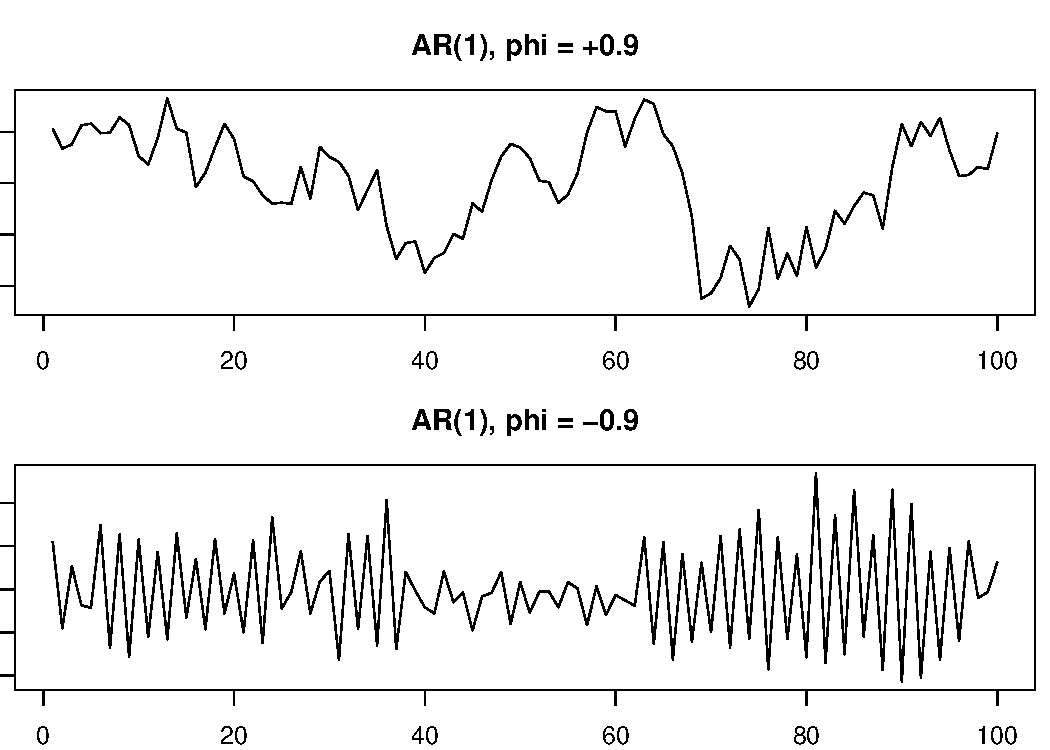
\includegraphics[width=0.85\textwidth]{fig/ar-1.pdf}
\caption{Two examples of AR(1) processes, with $\phi = \pm 0.9$.}
\label{fig:ar}
\end{figure}

\subsection{AR(1): auto-covariance and stationarity}

\begin{itemize}
\item A key question for us will be: \emph{under what conditions does the AR
    model  in \eqref{eq:ar-p}, or equivalently \eqref{eq:ar-p-phi}, define a
    stationary process?} 

\item The answer will turn out to be fairly sophisticated, but we can glean some
  intuition by starting with the AR(1) case: 
  \begin{equation}
  \label{eq:ar-1}
  x_t = \phi x_{t-1} + \epsilon_t 
  \end{equation}
  for  $t = 0, \pm 1 \pm 2, \pm 3,\dots$ 

\item Unraveling the iterations, we get
  \begin{align*}
  x_t &= \phi^2 x_{t-2} + \phi \epsilon_{t-1} + \epsilon_t \\
  &= \phi^3 x_{t-3} + \phi^2 \epsilon_{t-2} + \phi \epsilon_{t-1} + \epsilon_t
    \\  
  &\vdots \\ 
  &= \phi^k x_{t-k} + \sum_{j=0}^k \phi^j \epsilon_{t-j} 
  \end{align*}

\item If $|\phi| < 1$, then we can send $k \to \infty$ in the last display to 
  get 
  \begin{equation}
  \label{eq:ar-1-stationary}
  x_t = \sum_{j=0}^\infty \phi^j \epsilon_{t-j} 
  \end{equation}
  This is called the \emph{stationary representation} of the AR(1) process
  \eqref{eq:ar-1} 

\item Why is it called this? We can compute the auto-covariance function,
  writing $\sigma^2 = \Var(\epsilon_t)$ for the noise variance, as: 
  \begin{align*}
  \Cov(x_t, x_{t+h}) &= \Cov\bigg( \sum_{j=0}^\infty \phi^j \epsilon_{t-j}, 
  \sum_{\ell=0}^\infty \phi^\ell \epsilon_{t+h-\ell} \bigg) \\
  &= \sum_{j,\ell=0}^\infty \phi^j \phi^\ell \Cov( \epsilon_{t-j},
    \epsilon_{t+h-\ell} ) \\
  &= \sum_{j=0}^\infty \phi^j \phi^{j+h} \sigma^2 \\
  &= \sigma^2 \phi^h \sum_{j=0}^\infty \phi^{2j} \\
  &= \sigma^2 \frac{\phi^h}{1 - \phi^2} 
  \end{align*}
  where we used the fact that \smash{$\sum_{j=0}^\infty b^j = 1/(1-b)$} for $|b|
  < 1$. Since the auto-covariance in the last line only depends on $h$, we can
  see that the AR(1) process is indeed stationary

\item To reiterate, the representation \eqref{eq:ar-1-stationary}, and the
  auto-covariance calculation just given, would have not been possible unless
  $|\phi| < 1$. This condition is required in order for the AR(1) process to
  have a stationary representation. We will see later that we can general this
  come up with a condition that applies to an AR($p$), and beyond
\end{itemize}

\subsection{Causality (no, not the usual kind)}

\begin{itemize}
\item In order to study what conditions on the coefficients render a general
  AR($p$) model \eqref{eq:ar-p} stationary, we will introduce a concept called
  \emph{causality} 

\item (This is a slightly unfortunate bit of nomenclature that seems to be
  common in the time series literature, but has really nothing to do with
  causality used in the broader sense in statistics. We will ... somewhat
  begrudgingly ... stick with the standard nomenclature in time series here) 

\item We say that a series $x_t$, $t = 0, \pm 1, \pm 2, \dots$ is \emph{causal}
  provided that it can be written in the form
  \begin{equation}
  \label{eq:causal}
  x_t = \sum_{j=0}^\infty \psi_j \epsilon_{t-j}
  \end{equation}
  for a white noise sequence $\epsilon_t$, $t = 0, \pm 1 \pm 2, \pm
  3,\dots$, and coefficients such that \smash{$\sum_{j=0}^\infty |\psi_j| < 
      \infty$}

\item You should think of this as a generalization of
  \eqref{eq:ar-1-stationary}, where we allow for arbitrary coefficients
  $\psi_0,\psi_1,\psi_2,\dots$, subject to a summability condition 

\item It is straightforward to check that causality actually implies
  stationarity: we can just compute the auto-covariance function in
  \eqref{eq:causal}, similar to the above calculation:
    \begin{align*}
  \Cov(x_t, x_{t+h}) &= \Cov\bigg( \sum_{j=0}^\infty \psi_j \epsilon_{t-j}, 
  \sum_{\ell=0}^\infty \psi_\ell \epsilon_{t+h-\ell} \bigg) \\
  &= \sum_{j,\ell=0}^\infty \psi_j \psi_\ell \Cov( \epsilon_{t-j},
    \epsilon_{t+h-\ell} ) \\
  &= \sigma^2 \sum_{j=0}^\infty \psi_j \psi_{j+h}
  \end{align*}
  The summability condition ensures that these calculations are well-defined and
  that the last display is finite. Since this only depends on $h$, we can see
  that the process is indeed stationary

\item Thus, to emphasize, causality actually tells us \emph{more} than
  stationary: it is stationary ``plus'' a representation a linear filter of past
  white noise variates, with summable coefficients

\item Note that when $\psi_j = \phi^j$, the summability condition
  \smash{$\sum_{j=0}^\infty |\psi_j| < \infty$} is true if and only if $|\phi| <
  1$. Hence what we actually proved above for AR(1) was that it is causal if and
  only if $|\phi| < 1$. And it is this condition---for causality---that we will
  actually generalize for AR($p$) models, and beyond 
\end{itemize}

\section{MA models}

MA(q)
Backshift notation 

\begin{itemize}
\item
\end{itemize}

\subsection{MA(1): non-uniqueness and invertibility}

\begin{itemize}
\item
\end{itemize}

\section{ARMA models}

ARMA(p,q)
Backshift notation

point out special cases: 
ARMA(0,0): white noise
ARMA(1,0): random walk 

\begin{itemize}
\item
\end{itemize}

\subsection{Parameter redundancy}

Parameter redundancy
Recap of problems

\subsection{Causality and invertibility}

Forget about causality entirely

\subsection{Difference equations}

Diff equations --> don't cover.
Auto-covariance

\subsection{Partial auto-correlation function}

\section{ARIMA models}

Stationarity and differencing
ARIMA(p,d,q)
Backshift notation
Seasonality extensions

\subsection{Parameter estimation}

complicated --> don't cover.

\subsection{Regression with correlated errors}

complicated --> mostly don't cover

\section{Forecasting}

\end{document}
